% $Header: /cvsroot/latex-beamer/latex-beamer/examples/beamerexample5.tex,v 1.22 2004/10/08 14:02:33 tantau Exp $

\documentclass[11pt]{beamer}

\usetheme{Darmstadt}

\usepackage{times}
\usefonttheme{structurebold}

\usepackage[english]{babel}
%\usepackage[portuges]{babel}
\usepackage{pgf,pgfarrows,pgfnodes,pgfautomata,pgfheaps}
\usepackage{amsmath,amssymb}
\usepackage[utf8]{inputenc}
%\usepackage[latin1]{inputenc}
\usepackage{graphicx}

\setbeamercovered{dynamic}

\newcommand{\Lang}[1]{\operatorname{\text{\textsc{#1}}}}

\newcommand{\Class}[1]{\operatorname{\mathchoice
  {\text{\sf \small #1}}
  {\text{\sf \small #1}}
  {\text{\sf #1}}
  {\text{\sf #1}}}}

\newcommand{\NumSAT}      {\text{\small\#SAT}}
\newcommand{\NumA}        {\#_{\!A}}

\newcommand{\barA}        {\,\bar{\!A}}

\newcommand{\Nat}{\mathbb{N}}
\newcommand{\Set}[1]{\{#1\}}

\pgfdeclaremask{tu}{beamer-tu-logo-mask}
\pgfdeclaremask{computer}{beamer-computer-mask}
\pgfdeclareimage[interpolate=true,mask=computer,height=2cm]{computerimage}{beamer-computer}
\pgfdeclareimage[interpolate=true,mask=computer,height=2cm]{computerworkingimage}{beamer-computerred}
\pgfdeclareimage[mask=tu,height=.5cm]{logo}{logounesp}

\logo{\pgfuseimage{logo}}

\title{An�lise Combinat�ria e Probabilidades}
\author{Ney Lemke}
\institute[IBB-UNESP]{%
    Departamento de F�sica e Biof�sica}
\date{ 2011}                                

\colorlet{redshaded}{red!25!bg}
\colorlet{shaded}{black!25!bg}
\colorlet{shadedshaded}{black!10!bg}
\colorlet{blackshaded}{black!40!bg}

\colorlet{darkred}{red!80!black}
\colorlet{darkblue}{blue!80!black}
\colorlet{darkgreen}{green!80!black}

\def\radius{0.96cm}
\def\innerradius{0.85cm}

\def\softness{0.4}
\definecolor{softred}{rgb}{1,\softness,\softness}
\definecolor{softgreen}{rgb}{\softness,1,\softness}
\definecolor{softblue}{rgb}{\softness,\softness,1}

\definecolor{softrg}{rgb}{1,1,\softness}
\definecolor{softrb}{rgb}{1,\softness,1}
\definecolor{softgb}{rgb}{\softness,1,1}

\newcommand{\Bandshaded}[2]{
  \color{shadedshaded}
  \pgfmoveto{\pgfxy(-0.5,0)}
  \pgflineto{\pgfxy(-0.6,0.1)}
  \pgflineto{\pgfxy(-0.4,0.2)}
  \pgflineto{\pgfxy(-0.6,0.3)}
  \pgflineto{\pgfxy(-0.4,0.4)}
  \pgflineto{\pgfxy(-0.5,0.5)}
  \pgflineto{\pgfxy(4,0.5)}
  \pgflineto{\pgfxy(4.1,0.4)}
  \pgflineto{\pgfxy(3.9,0.3)}
  \pgflineto{\pgfxy(4.1,0.2)}
  \pgflineto{\pgfxy(3.9,0.1)}
  \pgflineto{\pgfxy(4,0)}
  \pgfclosepath
  \pgffill

  \color{black}  
  \pgfputat{\pgfxy(0,0.7)}{\pgfbox[left,base]{#1}}
  \pgfputat{\pgfxy(0,-0.1)}{\pgfbox[left,top]{#2}}
}

\newcommand{\Band}[2]{
  \color{shaded}
  \pgfmoveto{\pgfxy(-0.5,0)}
  \pgflineto{\pgfxy(-0.6,0.1)}
  \pgflineto{\pgfxy(-0.4,0.2)}
  \pgflineto{\pgfxy(-0.6,0.3)}
  \pgflineto{\pgfxy(-0.4,0.4)}
  \pgflineto{\pgfxy(-0.5,0.5)}
  \pgflineto{\pgfxy(4,0.5)}
  \pgflineto{\pgfxy(4.1,0.4)}
  \pgflineto{\pgfxy(3.9,0.3)}
  \pgflineto{\pgfxy(4.1,0.2)}
  \pgflineto{\pgfxy(3.9,0.1)}
  \pgflineto{\pgfxy(4,0)}
  \pgfclosepath
  \pgffill

  \color{black}  
  \pgfputat{\pgfxy(0,0.7)}{\pgfbox[left,base]{#1}}
  \pgfputat{\pgfxy(0,-0.1)}{\pgfbox[left,top]{#2}}
}

\newcommand{\BaenderNormal}
{%
  \pgfsetlinewidth{0.4pt}
  \color{black}
  \pgfputat{\pgfxy(0,5)}{\Band{input tapes}{}}
  \pgfputat{\pgfxy(0.35,4.6)}{\pgfbox[center,base]{$\vdots$}}
  \pgfputat{\pgfxy(0,4)}{\Band{}{}}

  \pgfxyline(0,5)(0,5.5)
  \pgfxyline(1.2,5)(1.2,5.5)
  \pgfputat{\pgfxy(0.25,5.25)}{\pgfbox[left,center]{$w_1$}}

  \pgfxyline(0,4)(0,4.5)
  \pgfxyline(1.8,4)(1.8,4.5)        
  \pgfputat{\pgfxy(0.25,4.25)}{\pgfbox[left,center]{$w_n$}}
  \ignorespaces}

\newcommand{\BaenderZweiNormal}
{%
  \pgfsetlinewidth{0.4pt}
  \color{black}
  \pgfputat{\pgfxy(0,5)}{\Band{Zwei Eingabeb�nder}{}}
  \pgfputat{\pgfxy(0,4.25)}{\Band{}{}}

  \pgfxyline(0,5)(0,5.5)
  \pgfxyline(1.2,5)(1.2,5.5)
  \pgfputat{\pgfxy(0.25,5.25)}{\pgfbox[left,center]{$u$}}

  \pgfxyline(0,4.25)(0,4.75)
  \pgfxyline(1.8,4.25)(1.8,4.75)        
  \pgfputat{\pgfxy(0.25,4.5)}{\pgfbox[left,center]{$v$}}
  \ignorespaces}

\newcommand{\BaenderHell}
{%
  \pgfsetlinewidth{0.4pt}
  \color{black}
  \pgfputat{\pgfxy(0,5)}{\Bandshaded{input tapes}{}}
  \color{shaded}
  \pgfputat{\pgfxy(0.35,4.6)}{\pgfbox[center,base]{$\vdots$}}
  \pgfputat{\pgfxy(0,4)}{\Bandshaded{}{}}

  \color{blackshaded}
  \pgfxyline(0,5)(0,5.5)
  \pgfxyline(1.2,5)(1.2,5.5)
  \pgfputat{\pgfxy(0.25,5.25)}{\pgfbox[left,center]{$w_1$}}

  \pgfxyline(0,4)(0,4.5)
  \pgfxyline(1.8,4)(1.8,4.5)        
  \pgfputat{\pgfxy(0.25,4.25)}{\pgfbox[left,center]{$w_n$}}
  \ignorespaces}

\newcommand{\BaenderZweiHell}
{%
  \pgfsetlinewidth{0.4pt}
  \color{black}
  \pgfputat{\pgfxy(0,5)}{\Bandshaded{Zwei Eingabeb�nder}{}}%
  \color{blackshaded}
  \pgfputat{\pgfxy(0,4.25)}{\Bandshaded{}{}}
  \pgfputat{\pgfxy(0.25,4.5)}{\pgfbox[left,center]{$v$}}
  \pgfputat{\pgfxy(0.25,5.25)}{\pgfbox[left,center]{$u$}}%

  \pgfxyline(0,5)(0,5.5)
  \pgfxyline(1.2,5)(1.2,5.5)

  \pgfxyline(0,4.25)(0,4.75)
  \pgfxyline(1.8,4.25)(1.8,4.75)        
  \ignorespaces}

\newcommand{\Slot}[1]{%
  \begin{pgftranslate}{\pgfpoint{#1}{0pt}}%
    \pgfsetlinewidth{0.6pt}%
    \color{structure}%
    \pgfmoveto{\pgfxy(-0.1,5.5)}%
    \pgfbezier{\pgfxy(-0.1,5.55)}{\pgfxy(-0.05,5.6)}{\pgfxy(0,5.6)}%
    \pgfbezier{\pgfxy(0.05,5.6)}{\pgfxy(0.1,5.55)}{\pgfxy(0.1,5.5)}%
    \pgflineto{\pgfxy(0.1,4.0)}%
    \pgfbezier{\pgfxy(0.1,3.95)}{\pgfxy(0.05,3.9)}{\pgfxy(0,3.9)}%
    \pgfbezier{\pgfxy(-0.05,3.9)}{\pgfxy(-0.1,3.95)}{\pgfxy(-0.1,4.0)}%
    \pgfclosepath%
    \pgfstroke%
  \end{pgftranslate}\ignorespaces}

\newcommand{\SlotZwei}[1]{%
  \begin{pgftranslate}{\pgfpoint{#1}{0pt}}%
    \pgfsetlinewidth{0.6pt}%
    \color{structure}%
    \pgfmoveto{\pgfxy(-0.1,5.5)}%
    \pgfbezier{\pgfxy(-0.1,5.55)}{\pgfxy(-0.05,5.6)}{\pgfxy(0,5.6)}%
    \pgfbezier{\pgfxy(0.05,5.6)}{\pgfxy(0.1,5.55)}{\pgfxy(0.1,5.5)}%
    \pgflineto{\pgfxy(0.1,4.25)}%
    \pgfbezier{\pgfxy(0.1,4.25)}{\pgfxy(0.05,4.15)}{\pgfxy(0,4.15)}%
    \pgfbezier{\pgfxy(-0.05,4.15)}{\pgfxy(-0.1,4.2)}{\pgfxy(-0.1,4.25)}%
    \pgfclosepath%
    \pgfstroke%
  \end{pgftranslate}\ignorespaces}

\newcommand{\ClipSlot}[1]{%
  \pgfrect[clip]{\pgfrelative{\pgfxy(-0.1,0)}{\pgfpoint{#1}{4cm}}}{\pgfxy(0.2,1.5)}\ignorespaces}

\newcommand{\ClipSlotZwei}[1]{%
  \pgfrect[clip]{\pgfrelative{\pgfxy(-0.1,0)}{\pgfpoint{#1}{4.25cm}}}{\pgfxy(0.2,1.25)}\ignorespaces}


\AtBeginSection[]{\frame{\frametitle{Outline}\tableofcontents[current]}}

\begin{document}

\frame{\titlepage}

%\section*{Outline}

\part{Parte I}
\frame{\frametitle{Outline}\tableofcontents[part=1]}
\section{Probabilidades}
\frame{\frametitle{Probabilidade}
Seja um conjunto $U$ com $N$ elementos seja um subconjunto $A$ com $n_A$ 
elementos. A probabilidade de ocorr�ncia de $A$ �
$$
p_A=\frac{n_A}{N}
$$

Exemplos:

\begin{itemize}
\item Dados
\item Cartas
\item Moedas
\end{itemize}

}

\frame{\frametitle{Eventos mutuamente Exclusivos}
Os eventos $A$ e $B$ s�o mutuamente exclusivos se a ocorr�ncia de $A$ impede a ocorr�ncia de $B$ e veice-versa. Ou seja se $A\cap B =\emptyset$.


}

\frame{\frametitle{Eventos Coletivamente Exaustivos}
Os eventos $A_1,\ldots ,A_n$ s�o coletivamente exaustivos se:

$$U=\cup_{i=1}^n A_i$$ 
}

\frame{\frametitle{Eventos Independentes}
Os eventos $A$ e $B$ s�o independentes se:

$$p_{A\cap B}=p_a p_B$$
}

\frame{\frametitle{Regra da soma}

  $$p(A \mbox { ou } B \ldots Z)=\frac{n_A+n_B+\ldots n_Z}{N}=p_A+p_B+\ldots p_Z$$
se os eventos s�o mutuamente exclusivos. 

}


\frame{\frametitle{Exemplo}
Qual � a probabilidade de se obter um dado 1 no primeiro lan�amentp ou um dado 4 no segundo?
}

\frame{\frametitle{Teorema}
$$p_{A\cup B}=p_A+p_B-p_{A\cap B}$$

}

\frame{\frametitle{Probabilidade Condicional}

$p(B|A)$ denotada a probabilidade de ocorr�ncia de $B$ dado que $A$ ocorreu.

Esta probabilidade pode ser calculada usando o teorema de Bayes:

$$p(A\cap B)=p(B|A)p(A)=p(A|B)p(B)$$

\begin{center}
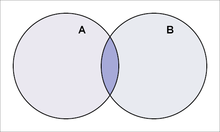
\includegraphics[scale=0.5]{intersec.png}
\end{center}

}
\section{An�lise Combinat�ria}

\frame{\frametitle{An�lise Combinat�ria}
  \begin{itemize}
  \item Permuta��es
  \item Arranjos
  \item Arranjos com Repeti��o
  \item Combina��es
  \end{itemize}
}


\frame{\frametitle{Permuta��es}

  Quantas listas ordenadas contendo $n$ elementos podemos formar a
  partir de uma lista com $n$ elementos diferentes.

$$n!$$
}

\frame{\frametitle{Arranjos}

  Quantas listas ordenadas contendo $p$ elementos podemos formar a
  partir de uma lista com $n$ elementos diferentes.

$$\frac{n!}{(n-p)!}$$
}


\frame{\frametitle{Arranjos com repeti��o}

  Quantas listas ordenadas contendo $n$ elementos podemos formar a
  partir de uma lista com $n$ elementos, onde o elemento $e_i$ aparece repetido
$r_i$ vezes.

$$\frac{n!}{r_1!\ldots r_n!}$$
}


\frame{\frametitle{Combina��es}

Quantos subconjuntos contendo $p$ elementos podemos construir com os elementos de um conjunto dom $n$ elementos?

$$C_{n,p}=\frac{n!}{p!(n-p)!}$$
}

\section{Caminhante Aleat�rio}


\frame{\frametitle{Caminhante Aleat�rio}

\begin{center}\includegraphics[scale=0.15]{rw}\end{center}

$N$ Passos

$N_1$ Passos para a frente

$N_2$ Passos para tr�s

Probabilidade de dar $N_1$ passos para a frente.
$$W_N(N_1)=\frac{N!}{N_1! (N-N_1)!} p^{N_1} q^{N-N_1}$$
}

\frame{\frametitle{Caminhante Aleat�rio}
Temos que:

$$\sum_{N_1=0}^N W_N(N_1)=\sum_{N_1=0}^N \frac{N!}{N_1! (N-N_1)!} p^{N_1} q^{N-N_1}=(p+q)^N=1$$

�  conveniente investigar a posi��o do caminhante $m=N_1-N_2$. Neste caso

$$W_N(m)=\frac{N!}{\left( \frac{N+m}{2}\right)!\left( \frac{N-m}{2}\right)!} p^{N_1} q^{N-N_1}$$
}

\frame{\frametitle{Equa��o Estoc�stica}

$$P_N(m)=pP_N(m-1)+q P_N(m+1)$$

Considere o caso $p=q=1/2$

$$\frac{P_{N+\tau}-P_N}{\tau}\sim \frac{\partial P}{\partial t}$$

$$\frac{P(ml-l)+P(ml+l)-2 P(ml)}{l^2}\sim \frac{\partial^2 P}{\partial x^2}$$

Equa��o da Difus�o:

$$\frac{\partial P}{\partial t}=D\frac{\partial^2 P}{\partial x^2}$$
}

\frame{\frametitle{Valores M�dios}
Seja $u_j$ uma vari�vel estoc�stica que pode assumir $N$ valores.

$$\sum^N P(u_j)=1$$

$$\langle u \rangle =\sum^Nu_jP(u_j)$$

$$(\Delta u)^2=(u-\langle u \rangle)^2=\langle u^2\rangle-\langle u\rangle^2 $$

}


\frame{\frametitle{Caminhante Aleat�rio}


$$\langle N_1 \rangle = \sum_{N_1} N_1 W_N(N_1)=\sum_{N_1} N_1 \frac{N!}{N_1! (N-N_1)!} p^{N_1} q^{N-N_1}$$

$$\langle N_1 \rangle = p\frac{\partial}{\partial p} \sum_{N_1} W_N(N_1)=\sum_{N_1} N_1 \frac{N!}{N_1! (N-N_1)!} p^{N_1} q^{N-N_1}$$

$$\langle N_1 \rangle=p\frac{\partial}{\partial p}(p+q)^N$$

$$\langle N_1 \rangle =pN(p+q)^{N-1}=pN$$

$$\langle N_2 \rangle=\langle N-N_1 \rangle=N(1-p)=Nq$$
}

\frame{\frametitle{Caminhante Aleat�rio}
$$\langle N_1^2 \rangle=p\frac{\partial}{\partial p}p\frac{\partial}{\partial p} \sum_{N_1}  W_N(N_1)=\sum_{N_1} N_1^2 \frac{N!}{N_1! (N-N_1)!} p^{N_1} q^{N-N_1}$$

$$\langle N_1^2 \rangle= p\frac{\partial}{\partial p}p\frac{\partial}{\partial p}(p+q)^N=pN+p^2N(N-1)$$

$$(\Delta N_1)^2=\langle N_1^2\rangle-\langle N_1\rangle^2 $$

$$(\Delta N_1)^2=pN+p^2N(N-1)-p^2N^2=Np(1-p)=Npq$$

$$\Delta N_1=\sqrt{Npq}$$
}

\frame{\frametitle{Lei dos Grandes N�meros}
$$\frac{\Delta N_1}{\langle N_1\rangle }=\sqrt{\frac{q}{pN}}$$
\begin{center}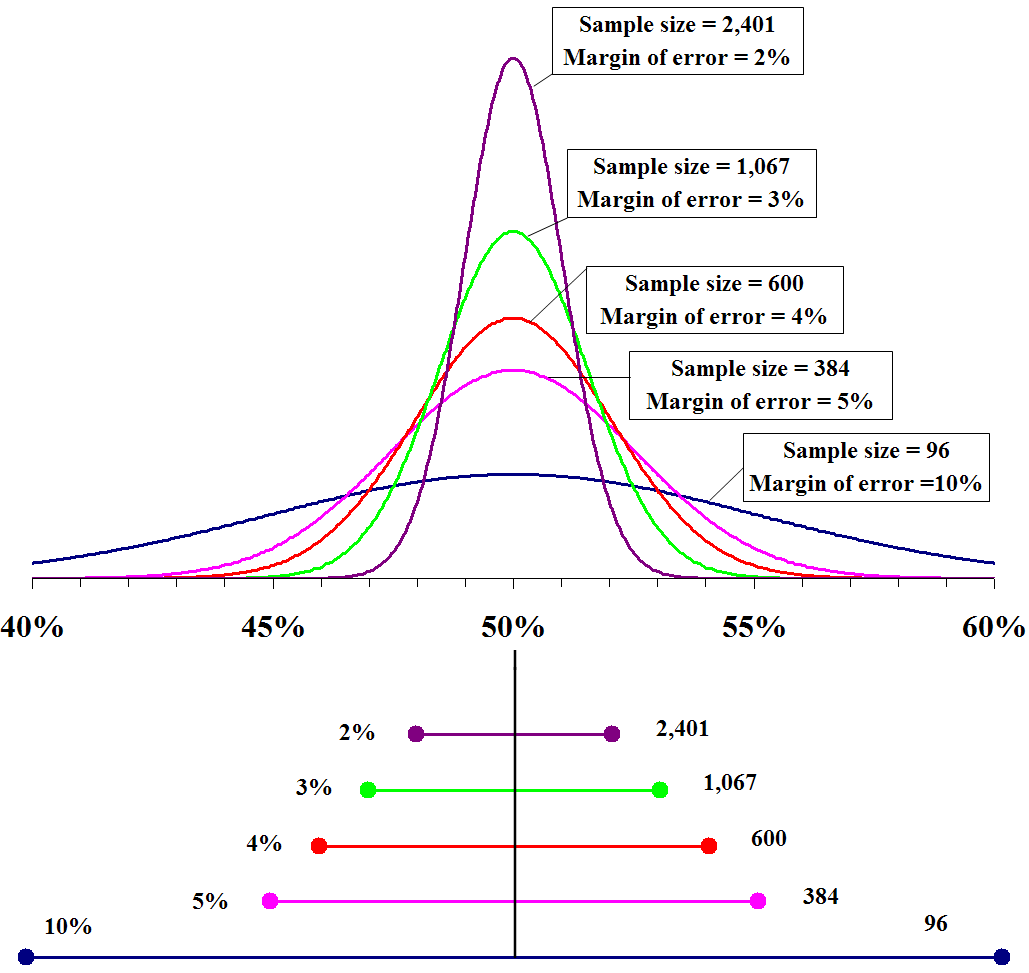
\includegraphics[scale=0.1]{lln.png}\end{center}

}


\frame{\frametitle{Aproxima��o de Stirling}

$$\ln N!=\ln 1+\ldots \ln N\sim \int_1^N \ln x\, d x=N \ln N -N +1\sim N\ln N -N $$


ou ainda 

$$N!\sim \sqrt{2\pi N}\left( \frac{N}{e} \right)^N$$

\begin{center}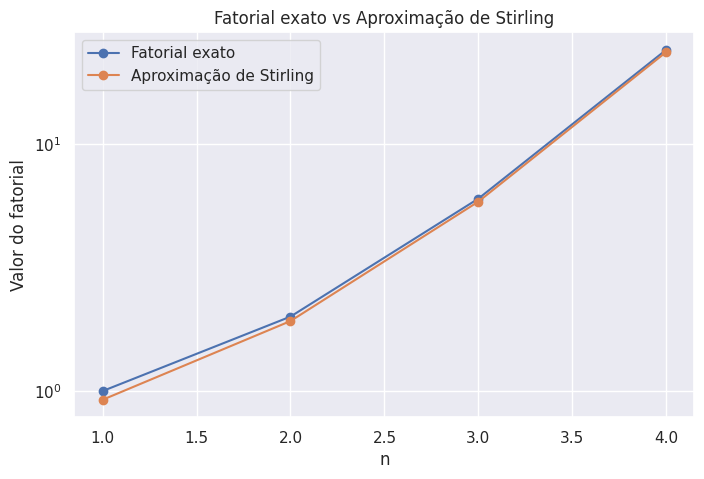
\includegraphics[scale=0.1]{stirling.png}\end{center}
}

\frame{\frametitle{Limite Gaussiano}

$$f(N_1)=\ln W_N(N_1) =ln N!-\ln N_1 - \ln N_2!+N_1\ln p+N_2 \ln q$$

Usando a aproxima��o de Stirling:

$$f(N_1)=N\ln N-N_1\ln N_1-(N-N_1)\ln (N-N_!)+N1\ln p +(N-N_1)\ln q$$

Expans�o em torno do m�ximo $N_1^*$:

$$f(N_1)\sim f(N_1^*)+(N_1-N_1^*)^2\left. \frac{1}{2}\frac{\partial^2 f}{\partial N_1^2}\right|_{N_1=N_1^*}+\ldots$$
}

\frame{\frametitle{Limite Gaussiano}
Equa��o para o m�ximo:

$$\frac{\partial f}{\partial N_1}=0$$

$$-\ln N_1^*+\ln (N_1-N_1^*)+\ln p-\ln q=0$$

$$N_1^*=N p$$
}
\frame{\frametitle{Limite Gaussiano}

Tamb�m precisamos calcular:

$$\frac{\partial^2 f}{\partial N_1^2}=\frac{1}{N-N_1}-\frac{1}{N_1}$$

$$\left. \frac{\partial^2 f}{\partial N_1^2}\right|_{N_1=N_1^*}=\frac{-1}{Npq}$$

$$f(N_1)\sim\ln W_N(N_1^*)-\frac{-(N_1-Np)^2}{2 Npq}$$

Normalizando temos que:

$$p(N_1)=\frac{1}{\sqrt{2 \pi N p q}}
\exp\left( \frac{-(N_1-Np)^2}{2 Npq}\right)$$
}

\end{document}


